\documentclass[10pt,border=4pt]{standalone}
\usepackage{mathptmx}
\usepackage{amsmath,amssymb,bm}
\usepackage{tikz}
\usetikzlibrary{patterns,decorations.pathmorphing,decorations.pathreplacing,arrows.meta,fit,backgrounds,calc,positioning,shapes.geometric}
\definecolor{acc}{HTML}{0B5394}
\definecolor{accl}{HTML}{EAF0F7}
\definecolor{grp}{HTML}{F5F5F5}
\definecolor{org}{HTML}{C55A11}
\definecolor{orgl}{HTML}{FBEFE6}
\tikzset{
 dat/.style={draw=black,line width=0.6pt,fill=white,align=center,font=\small,inner sep=3pt,minimum height=0.85cm},
 lay/.style={draw=acc,line width=0.8pt,fill=accl,rounded corners=2pt,align=center,font=\small,inner sep=3pt,minimum height=0.85cm},
 cnd/.style={draw=org,line width=0.8pt,fill=orgl,rounded corners=2pt,align=center,font=\small,inner sep=3pt,minimum height=0.75cm},
 op/.style={circle,draw=black,line width=0.6pt,fill=white,inner sep=0.5pt,font=\small,minimum size=5mm},
 grpb/.style={draw=black!45,dashed,line width=0.6pt,rounded corners=3pt,inner sep=6pt},
 arr/.style={-{Latex[length=2.2mm,width=1.7mm]},line width=0.7pt},
 carr/.style={-{Latex[length=2.2mm,width=1.7mm]},line width=0.7pt,draw=org},
 shp/.style={font=\scriptsize,text=black!70,inner sep=1pt},
 lab/.style={font=\footnotesize,inner sep=1pt},
 ttl/.style={font=\small\bfseries,inner sep=0pt,anchor=west}
}
\newcommand{\xh}{\mathbf{x}_h}\newcommand{\xf}{\mathbf{x}_f}

\definecolor{red}{HTML}{B3261E}
\tikzset{vv/.style={circle,draw=org,line width=0.9pt,fill=orgl,minimum size=1.25cm,font=\scriptsize,inner sep=0pt},
 vg/.style={circle,draw=black!70,line width=0.9pt,fill=black!25,minimum size=1.25cm,font=\scriptsize,inner sep=0pt},
 acc/.style={fill=red,draw=black,line width=0.4pt,minimum size=3mm,inner sep=0pt}}
\begin{document}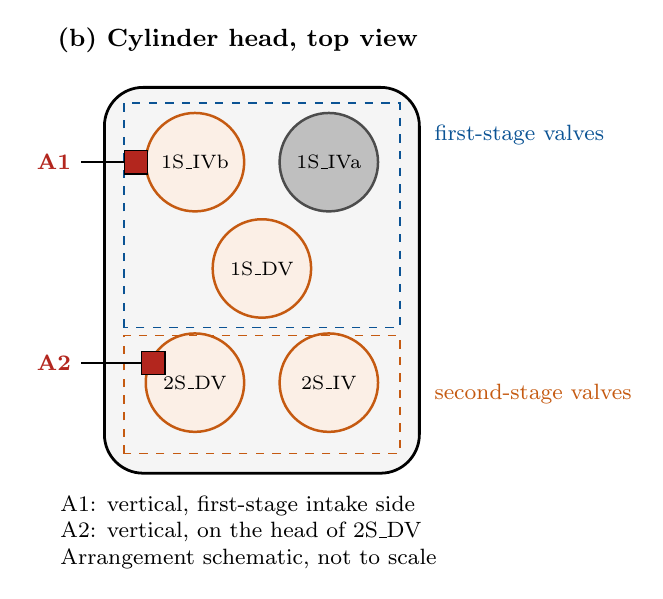
\begin{tikzpicture}[x=1cm,y=1cm]
\node[ttl] at (-2.6,2.9) {(b) Cylinder head, top view};
\draw[line width=1pt,fill=grp,rounded corners=14pt] (-2.0,-2.6) rectangle (2.0,2.3);
\node[vv] (ivb) at (-0.85,1.35) {1S\_IVb}; \node[vg] (iva) at (0.85,1.35) {1S\_IVa};
\node[vv] (dv1) at (0,0) {1S\_DV};
\node[vv] (dv2) at (-0.85,-1.45) {2S\_DV}; \node[vv] (iv2) at (0.85,-1.45) {2S\_IV};
\draw[dashed,acc!80,line width=0.6pt,draw=acc] (-1.75,-0.75) rectangle (1.75,2.1); \node[lab,anchor=west,text=acc] at (2.15,1.7) {first-stage valves};
\draw[dashed,line width=0.6pt,draw=org] (-1.75,-2.35) rectangle (1.75,-0.85); \node[lab,anchor=west,text=org] at (2.15,-1.6) {second-stage valves};
\node[acc] (a1) at (-1.6,1.35) {}; \draw[line width=0.5pt] (a1.west)--(-2.3,1.35) node[font=\footnotesize\bfseries,text=red,anchor=east]{A1};
\node[acc] (a2) at (-1.38,-1.2) {}; \draw[line width=0.5pt] (a2.west)--(-2.3,-1.2) node[font=\footnotesize\bfseries,text=red,anchor=east]{A2};
\node[lab,align=left,anchor=north west] at (-2.6,-2.85) {A1: vertical, first-stage intake side\\A2: vertical, on the head of 2S\_DV\\Arrangement schematic, not to scale};
\end{tikzpicture}\end{document}
